\documentclass[xcolor=pdftex,dvipsnames,table,mathserif,aspectratio=169]{beamer}
\usetheme{default}
\usetheme{metropolis}
\usepackage{minted}
\usepackage{mathtools}
\setbeamersize{text margin left=.3in,text margin right=.3in} 

\DeclarePairedDelimiter\abs{\lvert}{\rvert}%
\DeclarePairedDelimiter\norm{\lVert}{\rVert}%

\usepackage[english]{babel}
\usepackage{pgf,pgfarrows,pgfnodes,pgfautomata,pgfheaps}
\usepackage{amsmath,amssymb,setspace,centernot}
\usepackage[latin1]{inputenc}
\usepackage{pgf,tikz}
\usepackage[T1]{fontenc}
\usepackage{relsize}
\usepackage{pdfpages}
\usepackage[absolute,overlay]{textpos} 


\newenvironment{reference}[2]{% 
  \begin{textblock*}{\textwidth}(#1,#2) 
      \footnotesize\it\bgroup\color{red!50!black}}{\egroup\end{textblock*}} 

\DeclareMathSizes{10}{10}{6}{6} 

\begin{document}
\title{Part 12: Trees, Boosting, and Bagging}
\author{Chris Conlon}
\institute{Applied Econometrics II}
\date{\today}

\frame{\titlepage}


\begin{frame}
\frametitle{Reading}
\begin{itemize}
\item Chapters 9,10,15 of \textit{Elements of Statistical Learning}
\end{itemize}
\end{frame}



\section{Trees}
\begin{frame}
\frametitle{Decision Trees}
Start with $y = f(x_i)$:
\begin{itemize}
\item Construct a \alert{tree} by \alert{splitting} the sample on an $x_i$.
\begin{itemize}
\item Choose the split to maximize the criterion function.
\item Choose the $x_i$ to maximize the criterion given the proposed split.
\end{itemize}
\item Which $x_i$ do we choose?
\begin{itemize}
\item There are $K$ possibilities. 
\item But how do we know which order to split?
\end{itemize}
\item Which split do we choose?
\begin{itemize}
\item This is usually single dimensional optimization.
\end{itemize}
\item Resulting problem is $NP$ hard.
\end{itemize}
\end{frame}

\begin{frame}
\frametitle{Decision Trees}
What kind of tree?
\begin{itemize}
\item \alert{Classification} Trees predict \alert{discrete} outcomes.
\item \alert{Regression} Trees predict \alert{continuous} outcomes.
\end{itemize}
\end{frame}


%\begin{frame}
%\frametitle{Decision Trees: Titanic Survival}
%\begin{center}
%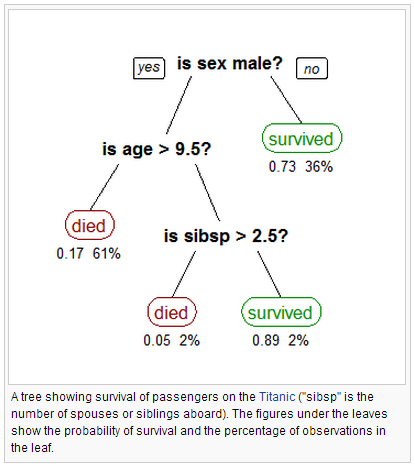
\includegraphics[width=2.5in]{./resources/titanic.png}
%\end{center}
%\end{frame}


\begin{frame}
\frametitle{Decision Trees: Covid Hospitalization (Petrilli et al 2020)}
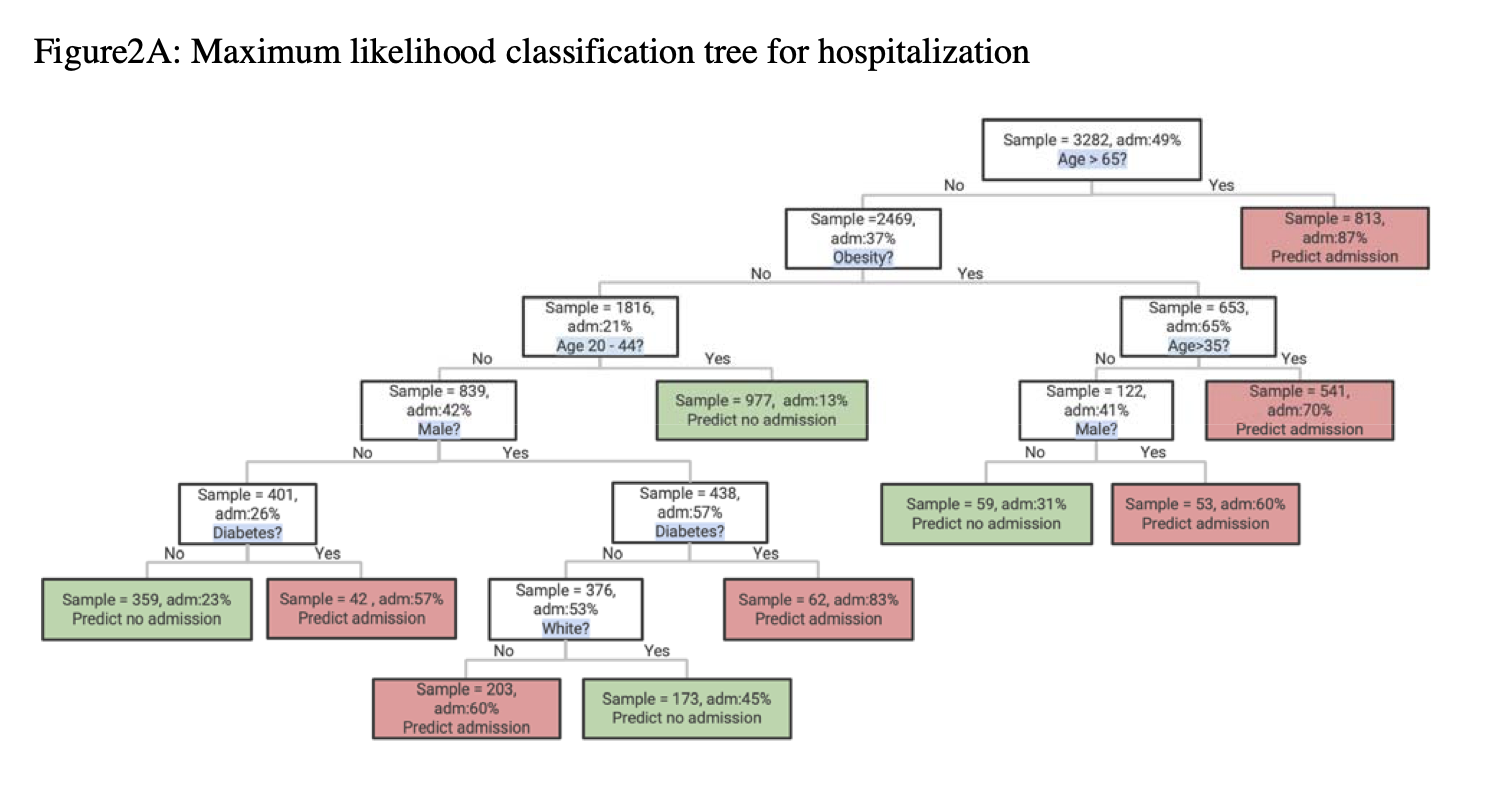
\includegraphics[width=5in]{./resources/covid_tree1.png}
\end{frame}


\begin{frame}
\frametitle{Decision Trees: Covid Critical Illness}
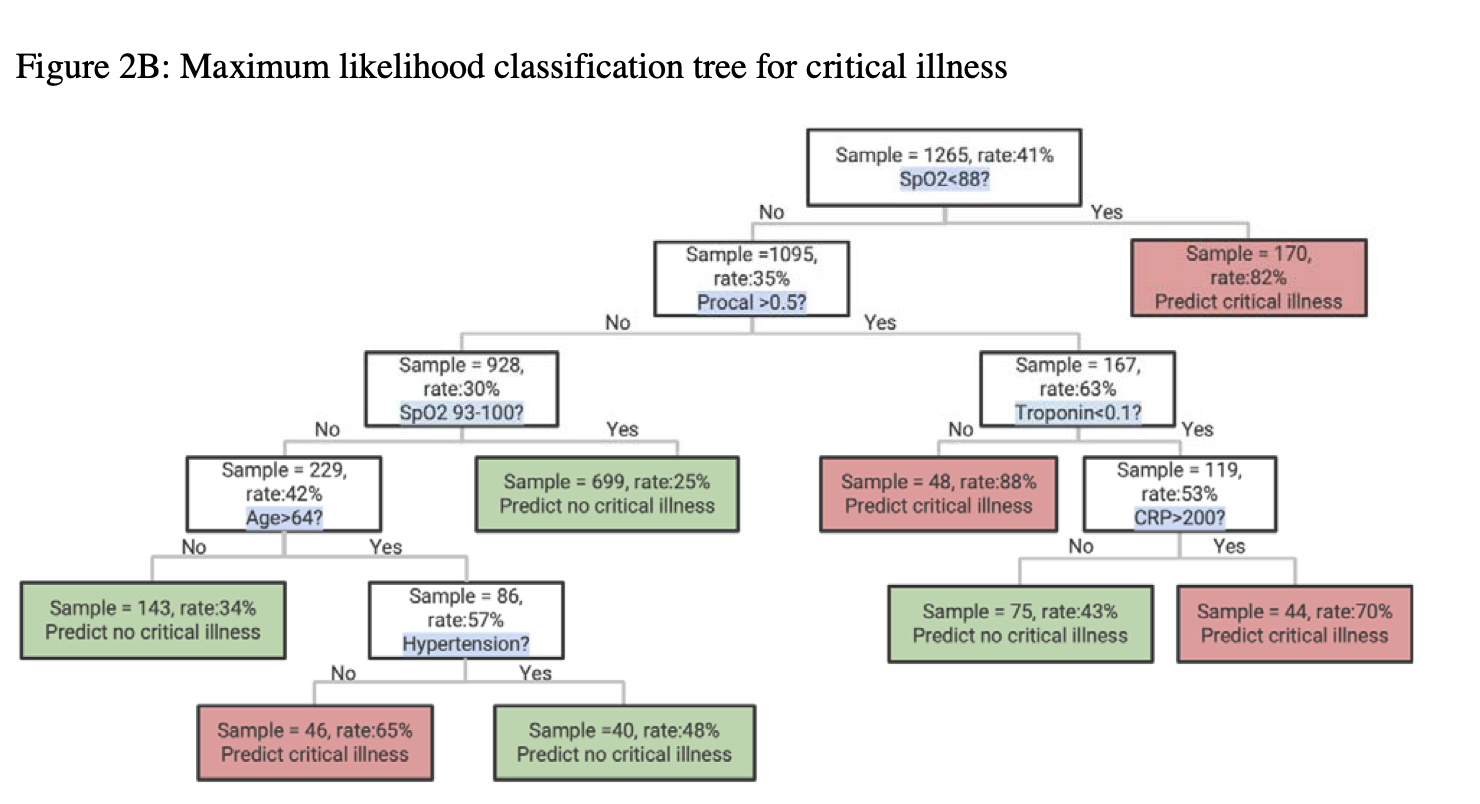
\includegraphics[width=5in]{./resources/covid_tree2.png}
\end{frame}

\section{How to choose splits?}

\begin{frame}
\frametitle{Decision Trees: Criteria \#1: RSS}
Residual sum of squares:
\begin{align*}
\min_f \sum_{i=1}^N (y - f(x_i))^2
\end{align*}
\begin{itemize}
\item ``Regression Trees''
\item Seems sensible for continuous $y$ not discrete $y$.
\item This is not OLS because $E[y | x]$ is \alert{highly nonlinear}.
\end{itemize}
\end{frame}

\begin{frame}
\frametitle{Decision Trees: Criteria \#2: Gini Impurity}
For each side of each split calculate (smaller is better):
\begin{align*}
\sum_j \underbrace{p_j}_{\text{Correct}} \times \underbrace{( \sum_{k \neq j} p_k )}_{\text{Incorrect}} =\sum_j p_j (1 -p_j) = 1 -\sum_j p_j^2 
\end{align*}
\begin{itemize}
\item 1265 Patients with 41\% Critical Rate $\rightarrow 0.2419$.
\item Split on $Sp02 < 88$
\begin{itemize} 
\item Left: 383 out of 1095 cases (35\%) $\rightarrow $ Gini: $0.2275$
\item Right: 140 out of 170 cases (82\%) $\rightarrow $ Gini: $0.1476$
\end{itemize}
\item Weighted avg: $\underbrace{(1095/1265)*(0.2275)}_{0.1968} + \underbrace{(140/1265)*(0.1476)}_{0.0163} = 0.2131$
\item Choose splits to minimze weighted average impurity.
\end{itemize}
\end{frame}



\begin{frame}
\frametitle{Decision Trees: Criteria \#3: Variance Reduction}
Calculate pre-split variance: $\underbrace{\frac{1}{|S|^{2}} \sum_{i \in S} \frac{1}{2}\left(y_{i}-y_{j}\right)^{2}}_{\text{Pre split Var}}$ and calculate post-split variance:
\begin{align*}
\underbrace{\frac{1}{\left|S_{t}\right|^{2}} \sum_{i \in S_{t}} \sum_{j \in S_{t}} \frac{1}{2}\left(y_{i}-y_{j}\right)^{2}}_{\text{Post split  TRUE}}
+\underbrace{\frac{1}{\left|S_{f}\right|^{2}} \sum_{i \in S_{f}} \sum_{j \in S_{f}} \frac{1}{2}\left(y_{i}-y_{j}\right)^{2}}_{\text{Post split FALSE}}
\end{align*}
\begin{itemize}
\item Maximize the \alert{reduction} in variance / minimize post-split variance
\item Note the connection, for discrete distribution $Var(y) = |S| \cdot p_j (1-p_j)$.
\end{itemize}
\end{frame}


\begin{frame}
\frametitle{Decision Trees: Criteria \#4: Information Gain/Entropy}
Start with the Kullback-Leibler divergence.
\begin{itemize}
\item This measures the distance between two distributions $P(x),Q(x)$.
\item If they are the same we get $\log(1) = 0$, otherwise expected log distance (where expectation over $p(x)$).
\begin{align*}
D_{\mathrm{KL}}(P \| Q)&=\sum_{x \in \mathcal{X}} P(x) \log_b \left(\frac{P(x)}{Q(x)}\right), \quad
D_{\mathrm{KL}}(P \| Q)=\int_{-\infty}^{\infty} p(x) \log_b \left(\frac{p(x)}{q(x)}\right) d x\\
%I G_{X, A}(X, a)&=D_{\mathrm{KL}}\left(P_{X}(x | a) \| P_{X}(x | I)\right)
\end{align*}
\item Should be $ \geq 0$ always.
\item Can write as $D_{\mathrm{KL}}(P \| Q)=-\sum_{x \in \mathcal{X}} P(x) \log_b \left(\frac{Q(x)}{P(x)}\right)$
\end{itemize}
%\item \alert{Information Gain} tells us how valuable how much divergence/entropy is reduced when observing $A=a$.
\end{frame}

\begin{frame}
\frametitle{Decision Trees: Criteria \#4: Information Gain/Entropy}
Derive the \alert{mutual information} and \alert{information gain} and \alert{entropy} $H(X)$:
\begin{align*}
I(X, Y) &\equiv K L(p(x, y) \| p(x) p(y))\\
 &= H(X)- H(X|Y)= H(Y)- H(Y|X)\\
 H(X) &= - \sum_{j=1}^J p_j \log_b p_j
\end{align*}
\begin{itemize}
\item Tells the divergence between $p(x,y)$ (joint distribution) and $p(x) p(y)$ (marginals).
\item Mutual information is symmetric, $KL$ divergence is not.
\item \alert{Information Gain} tells us how valuable how much divergence/entropy is reduced when observing $A=a$.
\end{itemize}
\end{frame}


\begin{frame}
\frametitle{Decision Trees: Criteria \#4: Information Gain/Entropy}
The same example:
\begin{itemize}
\item 1265 Patients with 41\% Critical Rate $\rightarrow  -0.41 \log_2 0.41 - 0.59 \log_2 0.59 = 0.9765 $
\item Split on $Sp02 < 88$
\begin{itemize} 
\item Left: 383 out of 1095 cases (35\%) $\rightarrow  -0.35 \log_2 0.35 - 0.65 \log_2 0.65 = 0.934 $
\item Right: 140 out of 170 cases (82\%) $\rightarrow  -0.82 \log_2 0.82 - 0.65 \log_2 0.18 = 0.68 $
\end{itemize}
\item Weighted avg: $\underbrace{(1095/1265)*(0.934)}_{0.866} + \underbrace{(140/1265)*(0.68)}_{0.134} = 0.900$
\end{itemize}
The goal is to maximize \alert{entropy reduction}.
\begin{align*}
IG(T,a) =   \underbrace{H(T)}_{0.9765} -\underbrace{H(T | a)}_{0.900} = 0.0765
\end{align*}
\end{frame}


\begin{frame}
\frametitle{What are trees actually doing?}
Think about the $RSS$ case : $\min_f \sum_{i=1}^N (y - f(x_i))^2$
\begin{itemize}
\item This is \alert{nonparametric regression}
\item It is also a \alert{kernel model}.
\item Partition the data: $\left\{R_{1}, \ldots, R_{M}\right\}$ into \alert{leaves} that are \alert{disjoint} and \alert{span the space} of $X$.
\item $ f(x)=\sum_{m=1}^{M} c_{m} 1\left(x \in R_{m}\right)$. 
\begin{itemize}
\item Where $c_m$ is mean of $y_i$ within leaf $R_m$.
\end{itemize}
\item This is just a \alert{locally constant} regression. But distance is not determined using bandwidth...
\item Alternative: $k$-NN where $k$ is the number of observations on same leaf.
\end{itemize}
\end{frame}


\begin{frame}
\frametitle{What are trees actually doing?}
When are trees the right tool?
\begin{itemize}
\item Because of multiple levels of splits: work best when true relationship is highly nonlinear.
\item Who has a heart attack?
\begin{itemize}
\item Lots of factors: high BP, overweight, age, family history, diabetes, etc.
\item  Logit:  these enter \alert{additively} in the index and increase \alert{log odds proportionally}.
\item Can interact multiple factors $highBP \times overweight$, etc.
\end{itemize}
\item If the true model is highly interacted: trees will do well.
\item In general trees have \alert{low bias} but \alert{high variance}
\begin{itemize}
\item Small changes in data can lead to wildly different splits (and trees).
\end{itemize}
\end{itemize}
\end{frame}


\begin{frame}
\frametitle{Linear vs. Nonlinear Relationships}
\begin{center}
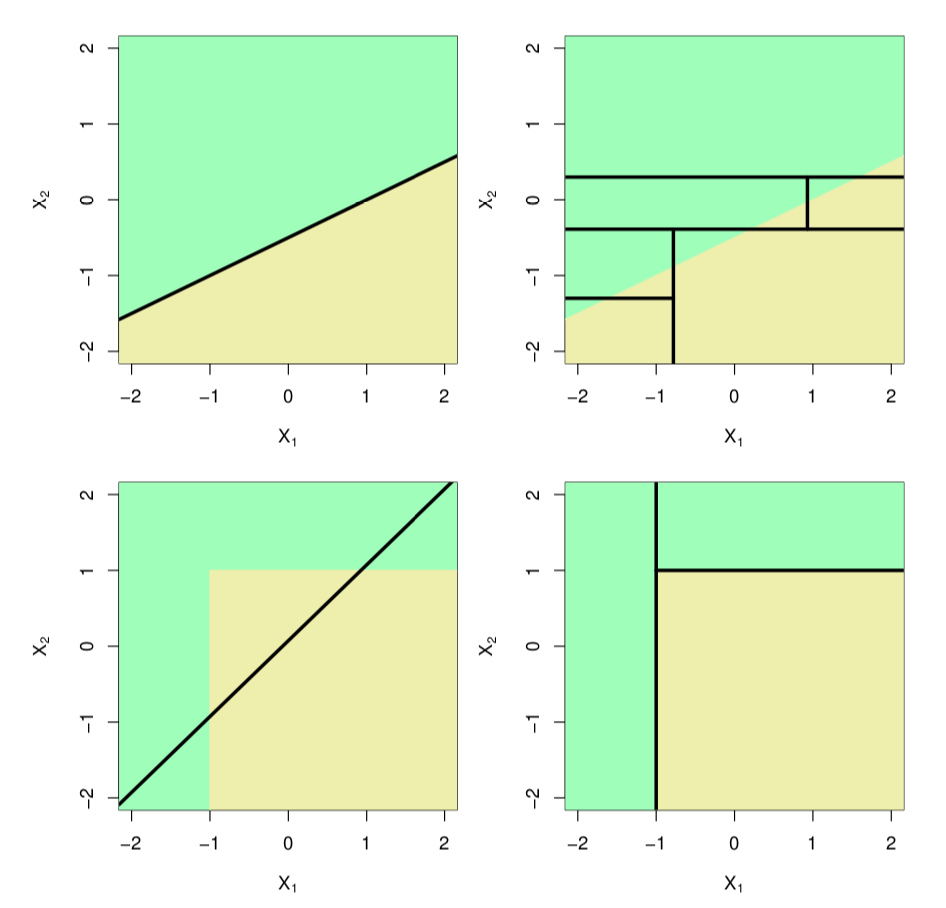
\includegraphics[width=3.5in]{./resources/treefit.png}
\end{center}
\end{frame}


\begin{frame}
\frametitle{How do splits work?}
\begin{itemize}
\item Binary variables: Trivial
\item Continuous Variables: Choose a split value $s$ so that $x>s$ or $x\leq s$ optimizes your criteria.
\begin{itemize}
\item This is a single dimensional search (Golden Section, etc.).
\end{itemize}
\item Multiple Categories $(A,B,C)$: this is the hard case
\begin{itemize}
\item Order by the outcome variable $y_b > y_a > y_c$.
\item Then treat like the continuous case.
\end{itemize}
\end{itemize}
\end{frame}

\begin{frame}{Growing your Tree}
\begin{itemize}
\item Let $|T| = M$ denote the number of terminal nodes in $T$ . We will use $|T|$ to measure the complexity of a tree. For any given complexity,
we want the tree minimizing square error on training set.
\item Finding the optimal binary tree of a given complexity is computationally intractable (NP hard).
\end{itemize}
\end{frame}


\begin{frame}{Tree Algorithms}
How do we build a tree?
\begin{itemize}
\item Because the problem is $NP$ hard: no ideal way.
\item Mostly heuristics.
\item Greedy Algorithm: Choose best split first for best $x$ go from there.
\begin{itemize}
\item Need not be optimal...
\end{itemize}
\item Avoiding \alert{over-fitting}
\begin{itemize}
\item How deep to make tree?
\item Minimum number of observations per branch?
\item Pruning?
\item Trees will always overfit if you let them!
\end{itemize}
\end{itemize}
\end{frame}

%
%\begin{frame}
%\frametitle{Overfitting: Bias Variance}
%\begin{center}
%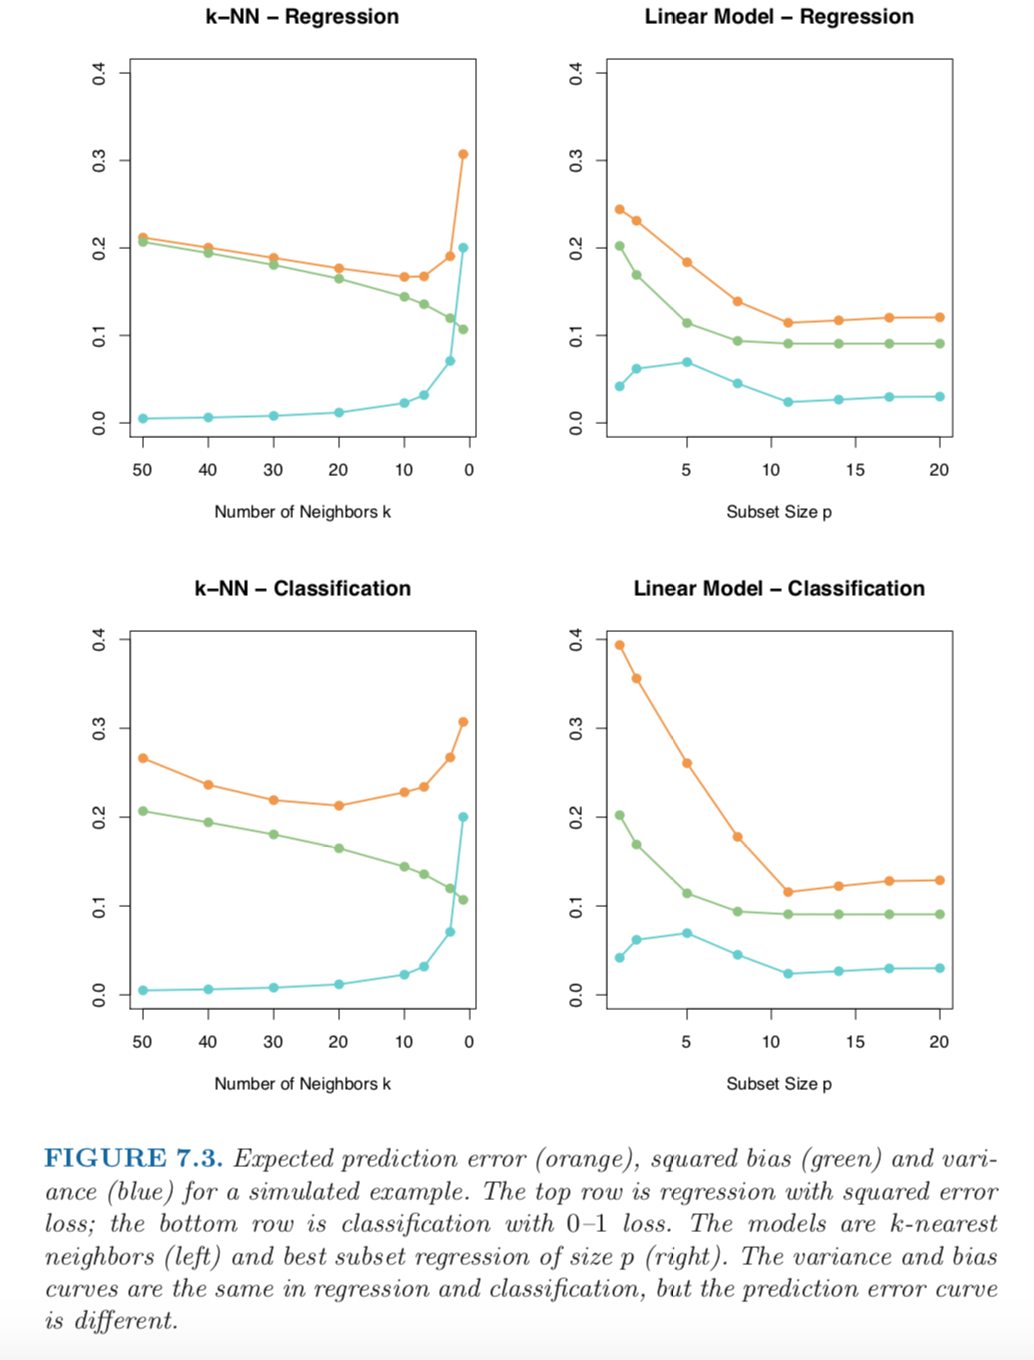
\includegraphics[width=2.35in]{./resources/bias-variance.png}
%\end{center}
%\end{frame}


\begin{frame}{Why Prune a Tree?}
To avoid overfitting
\begin{itemize}
\item Any useful split will be made (eventually).
\item We (may) end up with perfectly predicted outcomes $E[y_i | x_i]$.
 case we know for sure that $y_i=1$ ?
\item Remove leaves with too few elements.
\item Usually use a hold-out sample (test set) and remove leaves if it increases OOS criteria.
\item Other canned pruning algorithms will generate several candidate \alert{subtrees}
\begin{itemize}
\item Used out of sample critieria to pick the best subtree
\end{itemize}
\item Can also do \alert{early stopping}
\end{itemize}
\end{frame}



\begin{frame}{Tree Algorithms}
About \alert{criteria} and \alert{heuristics}.
\begin{itemize}
\item ID3 (Iterative Dichotomiser 3)
\item C4.5 (successor of ID3)
\item CART (Classification And Regression Tree)
\item Chi-square automatic interaction detection (CHAID). Performs multi-level splits when computing classification trees.
\item MARS: extends decision trees to handle numerical data better.
\item Conditional Inference Trees. Statistics-based approach that uses non-parametric tests as splitting criteria, corrected for multiple testing to avoid overfitting. This approach results in unbiased predictor selection and does not require pruning.
\end{itemize}
\end{frame}



\section{Bagging}
\begin{frame}{Bagging}
What is \alert{Bagging}? \alert{B}ootstrap \alert{Agg}regation.
\begin{itemize}
\item We re-sample a new dataset the size of our original dataset \alert{with replacement}
\item Before we re-ran our estimation to get $\hat{\theta}^b$ and took $Var(\hat{\theta}^{(1)},\hat{\theta}^{(2)},\ldots,\hat{\theta}^{(B)})$ and $E(\theta)=\frac{1}{B} \sum_{b=1}^B \hat{\theta}^b$.
\item Since we are doing ML, let's bag $\hat{y}_i$.
\item $E(y )=\frac{1}{B} \sum_{b=1}^B \hat{y}^b$ (we could also do this conditionally).
\end{itemize}
\end{frame}

\begin{frame}{Bagging: What's the point?}
Why would we want to do this?
\begin{itemize}
\item If we are worried about high-variance and \alert{overfitting} bagging will reduce our variance.
\item Each bootstrapped sample $b$ is like an IID realization of our data.
\item Averaging over  samples can reduce the variance of $\hat{y}$ by $\frac{1}{B}$.
\end{itemize}
The problem \alert{Interpretability}
\begin{itemize}
\item If my ``model'' is OLS I can report average coefficients.
\item If my model is a tree, what do I even report averaged over 1000 bootstrapped simulations?
\end{itemize}
\end{frame}

\begin{frame}{How to interpret variables?}
\begin{itemize}
\item Pick a tree $T^b$ calculate how much a particular variable $x_1$ increases the Gini Index, or decreases RSS, etc.
\item Average over all trees (some trees will be zero if they don't include $x_1$).
\item Report the average in \alert{relative} terms for all $x_k$.
\end{itemize}

\end{frame}


\begin{frame}
\frametitle{Variable Importance Plots}
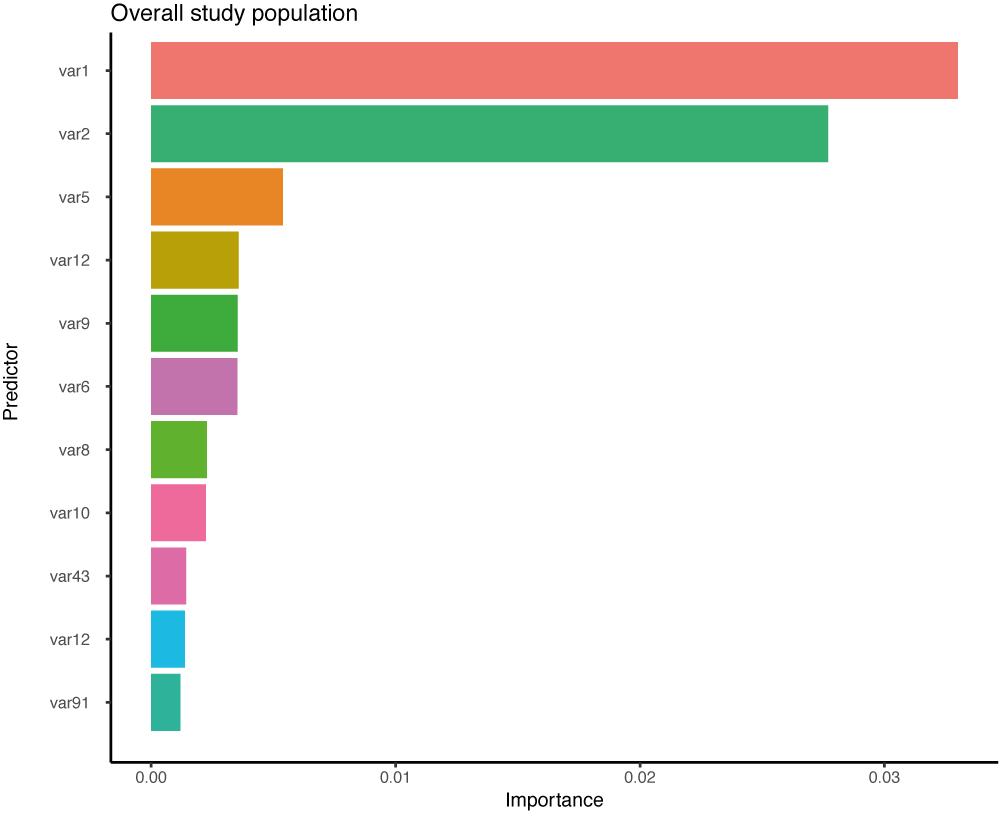
\includegraphics[width=3.8in]{./resources/Importance.jpg}
\end{frame}

\begin{frame}
\frametitle{Variable Importance Plots}
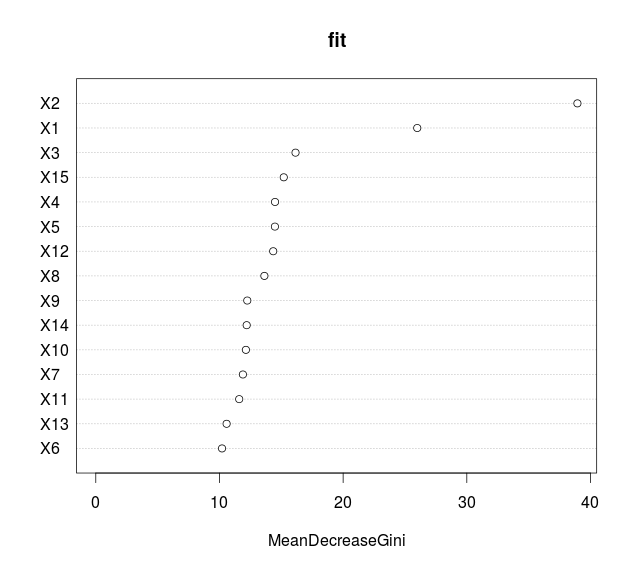
\includegraphics[width=3.8in]{./resources/variable-importance.png}
\end{frame}


\begin{frame}{Validation: How do assess model fit?}
Out of Bag Error Rate (OOB)
\begin{itemize}
\item Use \alert{cross validation}
\item Draw a bootstrap sample of size $N$.
\item Split sample into two parts: training $\frac{2}{3}$, validation $\frac{1}{3}$
\item Fit on the training sample
\item Predict on the validation sample: $(y_i - \hat{y}_i^{OOB})^2$
\item Report average or (mean-squared) error on the validation sample only.
\item Gives us expected out of sample fit.
\end{itemize}
Is this the same as error rate on totally new data?
\end{frame}

\begin{frame}
\frametitle{Bagging: OOB error}
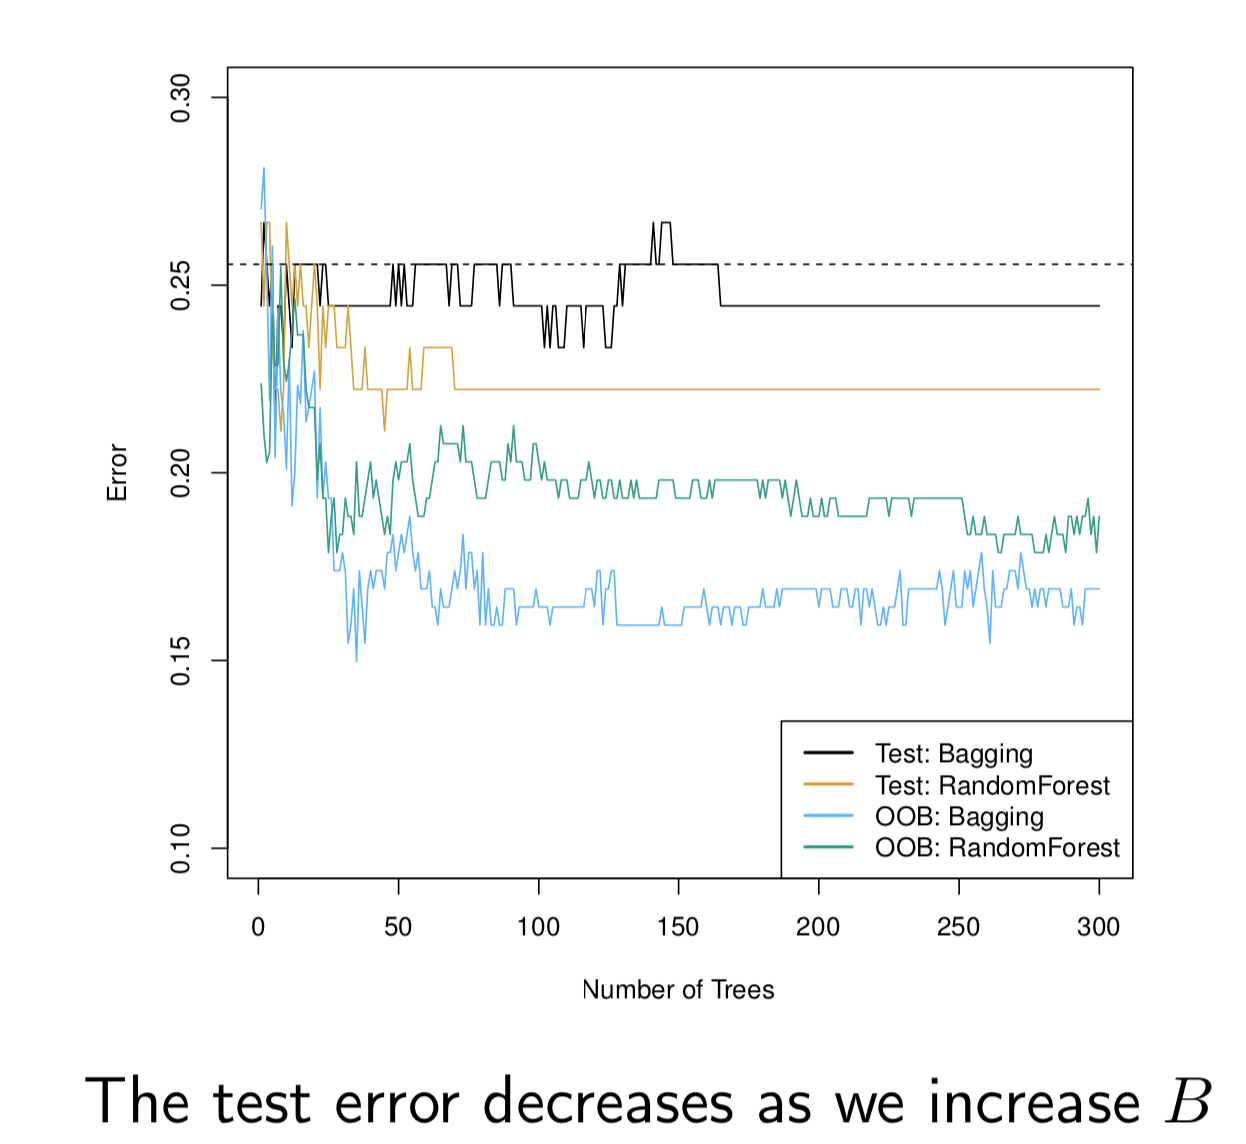
\includegraphics[width=4in]{./resources/bagging.png}
\end{frame}

\begin{frame}
\frametitle{Why do Bagging do so poorly?}
\begin{itemize}
\item Even though we bootstrap our sample many times $\rightarrow$ $(T^B,T^{B'})$ are highly correlated.
\item Why does this happen?
\begin{itemize}
\item We end up with the same $X$'s and the same splits in each model.
\end{itemize}
\item Adding more trees doesn't really improve forecast performance.
\item We would like to add more trees but have them be \alert{less correlated} with one another.
\end{itemize}
\end{frame}


\begin{frame}
\frametitle{Solution: Random Forests}
\begin{enumerate}
\item Draw a bootstrap sample $b$.
\item Fit a tree (usually a small one with limited depth)
\item At each node select a \alert{random subset} of regressors $m < K$ from $X$.
\item Average the predictions of (hopefully) less correlated trees. (Or Majority Vote).
\end{enumerate}
How to choose $m$? Usually $\sqrt{K}$.
\end{frame}



\begin{frame}
\frametitle{Solution: Random Forests}
\begin{itemize}
\item Even though we bootstrap our sample many times $\rightarrow$ $(T^B,T^{B'})$ are highly correlated.
\item Adding more trees doesn't really improve forecast performance.
\item We would like to add more trees but have them be \alert{less correlated} with one another.
\end{itemize}
\end{frame}

\begin{frame}{Evaluating Random Forests}
How important is $X^{(j)}$? Look at the trees that randomly don't include it in $m$ (or don't select it)
\begin{align*}
\widehat{\Delta}_{j}=\frac{1}{m} \sum_{i \in \mathcal{H}} \left(Y_{i}-\widehat{m}_{(-j)}\left(X_{i}\right)\right)^{2}-\left(Y_{i}-\widehat{m}\left(X_{i}\right)\right)^{2}
\end{align*}
Average this quantity across the entire training set:
\begin{align*}
\mathbb{E}\left[\widehat{\Delta}_{j} | \mathcal{T}\right]=\mathbb{E}\left[\left(Y-\widehat{m}_{(-j)}(X)\right)^{2}-(Y-\widehat{m}(X))^{2} | \mathcal{T}\right] \equiv \Delta_{j}
\end{align*}
This is called \alert{Leave-One-Out-COvariates} (LOCO).
\end{frame}


\begin{frame}{Inference on Random Forests}
\begin{itemize}
\item Technically possible but tricky
\item Active area of research
\item See Wager and Athey (2017).
\end{itemize}
\end{frame}




\begin{frame}{What about Boosting?}
\begin{enumerate}
\item Set $\hat{f}(x) = 0$ and $r_i = y_i$ for $i=1,\ldots, N$.
\item For $b=1,\ldots,B$ iterate on:
\begin{enumerate}
\item Fit a tree $\hat{f}^b$ with $d$ splits to the response $r_1,\ldots, r_n$.
\item Update the prediction to
\begin{align*}
\hat{f}(x) \leftarrow \hat{f}(x)+\lambda \hat{f}^{b}(x)
\end{align*}
\item Update the residual
\begin{align*}
r_{i} \leftarrow r_{i}-\lambda \hat{f}^{b}\left(x_{i}\right)
\end{align*}
\end{enumerate}
\item Produce the final model by averaging
\begin{align*}
\hat{f}(x)=\sum_{b=1}^{B} \lambda \hat{f}^{b}(x)
\end{align*}
\end{enumerate}
\end{frame}


\begin{frame}{How does Boosting Work?}
\begin{itemize}
\item At each bootstrap iteration we aren't fitting $y_i$
\item We are fitting $r_i$ the residual $y_i - \sum_{b'=1}^{b} \lambda \hat{f}^{b'}$. 
\item $\lambda$ is usually small so that we update the model \alert{slowly}.
\item You can think about what we are doing as \alert{re-weighting our training data}
\begin{itemize}
\item Put more weight on the cases we fit the worst (large residuals).
\end{itemize}
\item Usually set $\lambda$ small $.01$
\item Well known algorithm \alert{AdaBoost}
\end{itemize}
Boosting $>$ Bagging $>$ Single Tree
\end{frame}

\begin{frame}{ AdaBoost: Freund \& Schapire, 1996}
\begin{enumerate}
\item Weight observations equally $w_i = \frac{1}{N}$. for all $i=1,\ldots,N$.
\item From $b=1,\ldots, B$ do the following:
\begin{enumerate}
\item Fit a model  $f^{(b)}(x_i)$ to training data using $w_i$.
\item Compute $err_b = \frac{\sum_{i=1}^N w_i I[ y_i \neq f^{(b)}(x_i) ]}{\sum_{i=1}^N w_i}$
\item Compute $\alpha_b = \log \left(  \frac{1-err_b}{err_b}\right)$
\item Update weights for $i=1,\ldots,N$: 
\begin{align*}
w_i \leftarrow w_i \cdot \exp[\alpha_b I (y_i \neq f^{(b)}(x_i)) ]
\end{align*}
renormalize so that $\sum w_i =1$.
\end{enumerate}
\item Compute $\hat{f}(x) = sign[ \sum_{b} \alpha_b \hat{f}^{(b)}(x_i)]$.
\end{enumerate}
\end{frame}


\begin{frame}{Additive Models}
\begin{itemize}
\item $\hat{f}(x) = \sum_{b} \alpha_b \hat{f}^{(b)}(x_i)$ is an \alert{additive model}
\item Lots of examples in the literature:
\begin{itemize}
\item  Basis Functions (ie: polynomials) $\sum_{k=1}^K \theta_k g_k(x)$.
\item GAMs: $f(x) = \sum_{k=1}^K f_k(x)$.
\end{itemize}
\item Usually we fit these in \alert{one step} (OLS, MLE, etc.)
\item Here we fit $\alpha_b, \theta_b$ in a \alert{stagewise} manner.
\item Process fits slowly but avoids overfitting problem.
\end{itemize}
\end{frame}




\begin{frame}{What about Gradient Boosting?}
Same as AdaBoost with some modifications
\begin{itemize}
\item Loss function $L(y_i,\gamma)$
\item Choose $\gamma$ to minimize $\min L(y_i,\gamma)$ and get $h_b(x)$.
\item Update $r_i = \left[ \frac{\partial L(y_i, F(x_i))}{ \partial F(x_i)} \right]$ this is the \alert{gradient} evaluated at $b$th iteration of $F_b(x_i)$.
\item Update $F_b(x) = F_{b-1}(x) + \gamma_b h_b(x)$.
\end{itemize}
\end{frame}


\begin{frame}{How do we do this in R?}
\begin{itemize}
\item Sample Splitting, Bagging, etc. \texttt{caret}, \texttt{sample}
\item Gradient Boosting. \texttt{gbm} (easy), \texttt{xgboost} (faster).
\item Random forest \texttt{randomForest}.
\end{itemize}
\end{frame}

\section{Thanks!}


\end{document}
